\section{Einleitung}

\section{Laufzeit}

\section{Dokumentation der Implementierung}

\subsection{Testen der ungeraden Knotengerade}

In einem Graphen mit mindestens einem Knoten, welcher einen ungeraden Knotengrad hat, kann der Hierholzer Algorithmus keinen Erfolg haben. Ein Beispiel ist hier\ref{fig:unevenGraph} in den Tests zu finden.\\

Um sicherzustellen, dass dem Algorithmus ein valider Graph übergeben wird, wurde folgende Methode implementiert:

\begin{lstlisting}[language = java, frame = trBL]
private static boolean graphIsValid(Graph graph) {
    ....
    List<Node> nodesWithFalseDegree = graph.nodes()
                            .filter(node -> node.getDegree() % 2 != 0)
                            .collect(Collectors.toList());        
    for(Node node: nodesWithFalseDegree) {
        if(node.getEdgeBetween(node.getId()) == null) {
            return false;
        }
    }
    ...
}
\end{lstlisting}

Um zu prüfen ob Knoten einen ungeraden Kantengrad haben, werden diese Knoten zuerst alle in einer Liste gespeichert. Das ist notwendig, denn durch die genutzte Graphstream Bibliothek ensteht folgendes Problem: Angenommen es existiert ein Graph mit einem Knoten A und zwei Nachbarknoten B und C. Der Knoten A hat eine Schleife. Der Graph ist vollständig - A,B und C sind also alle miteinander verbunden (Abb. \ref{fig:loop}). 

\begin{figure}[htbp]
	\centering
		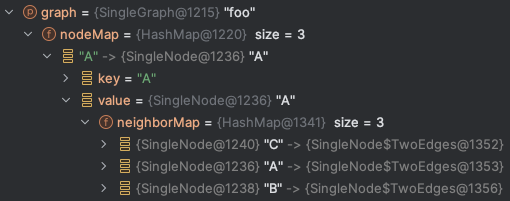
\includegraphics[width=0.6\textwidth]{Latex/Figs/loopedGraphDebugger.png}		
	\caption{Ausschnitt des Graphen mit Loop aus dem Debugger}
	\label{fig:loopedGraphDebugger}
\end{figure}

Wie nun im Debugger zu sehen\ref{fig:loopedGraphDebugger} hat der Knoten A nun nur drei Nachbarn. Zusätzlich hat er auch nur drei adjazente Kanten, AA, AB und AC. Das ist soweit alles korrekt. Der daraus resultierende Knotengrad ist allerdings ungerade und würde diesen Graph als invalide auswerten. Bei Betrachtung des Graphen hat dieser aber einen geraden Knotengrad.\\
Um dieses Problem zu umgehen wird in allen Kanten mit ungeradem Knotengrad also zusätzlich geprüft ob diese Kanten keine Schleifen sind. Erst wenn das der Fall ist, wird der Graph als invalide ausgewertet.